\documentclass[12pt, a4paper]{article}

\usepackage[T1]{fontenc}
\usepackage[utf8]{inputenc}
\usepackage[italian]{babel}
\usepackage{graphicx}
\graphicspath{ {img/} }

\usepackage{multirow}
\usepackage{hyperref}

\begin{document}

    \begin{titlepage}
        \begin{center}
            Indirizzo del sito: http://tecweb2021.studenti.math.unipd.it/cmichele \\
            \textbf{Autori} \\
            christian.micheletti@studenti.unipd.it (referente) \\
            jacopo.fichera@studenti.unipd.it \\
            \textbf{Repository pubblica} \\
            https://github.com/MicheGit/ProgettoTecweb
            \vfill
            Gli account utente usano una e-mail per effettuare l'accesso. Fanno eccezione le seguenti coppie: \\
            user / user \\
            admin / admin
        \end{center}
    \end{titlepage}

    \newpage

    \tableofcontents

    \newpage

    \begin{abstract}
        BirdWatchers è un sito dedicato a esperti e dilettanti, in generale, agli appassionati del birdwatching. Lo scopo di questo sito è quello di raccogliere e catalogare avvistamenti di uccelli da parte degli utenti e dar loro uno spazio dove discuterne.
    \end{abstract}

    \newpage


    \section{Analisi}

    \subsection{Utenza}
    Il sito web realizzato si rivolge a tutti coloro sono appassionati o intendono avvicinarsi al Birdwatching.
    Essendo un'attività diffusa principalmente tra persone oltre la mezza età, infatti in diversi censimenti
    in suolo statiunitense gli appassionati appartenenti ad una fascia di età minore dei 44 anni è sempre stata sotto il 39\%
    con un lieve incremento negli ultimi anni\footnote{Studi e dati riportati nelle fonti.},
    ci permette di  considerare che il traffico sulla pagina sarà ampiamente
    influenzato da persone con possibilmente poca dimestichezza tecnologica, favorendo la scelta di la sviluppare
    un'interfaccia e un set di funzionalità più intuitivo e semplice possibile.
    Gli utenti si troveranno sulla piattaforma per condividere la loro esperienza e conoscere altre persone che
    condividono la loro stessa passione, fornendo quindi uno spazio libero a tutti per creare amicizie e a
    mbienti di collaborazione tra diverse persone del mondo.
    \subsubsection{Interessati}
    Chiamiamo gli interessati coloro che non hanno grande conoscenza del mondo del Birdwatching e intendono scoprirne di più.
    Loro non hanno un obbiettivo mirato e si fanno guidare dalla presentazione dei contenuti, come il catalogo delle specie
    raccolte sul sito o quelle che sono le attività più popolari condivise dagli utenti più esperti.
    \subsubsection{Appassionati}
    Gli appassionati sono coloro che danno vita al cuore del sito in quanto saranno i più attivi nella pubblicazione
    di contenuti e nell'interazione con altri utenti.
    Potrà essere di loro interesse voler cercare dei contenuti più mirati tra i post pubblicati o il catalogo stesso
    per approfondire le loro conoscenze o risolvere uno specifico problema che potrebbe aver riscontrato qualcun altro.
    
    \subsubsection{Esperti}
    Esperti del mondo del Birdwatching si comporteranno come gli appassionati fornendo con molta probabilità risposte
    della comunità o magari contenuti di rilievo maggiore.

    \section{Progettazione}
    Come strategia di progettazione abbiamo seguito la \textit{responsive web design}, definendo dal principio solo i componenti necessari alle singole pagine. Abbiamo quindi sviluppato un piccolo framework orientato agli oggetti: i componenti presentano diversi livelli di genericità, in modo da favorirne il riuso, prerogativa cruciale per un sito web quasi totalmente dinamico.
    È stato scelto XHTML per via della sua rigida aderenza agli standard web, che assicura la compatibilità con la stragrande maggioranza dei browser, tuttavia in corso d'opera abbiamo deciso di cambiare in HTML5. Invece di utilizzare i tag peculiari di HTML5, per assicurare la compatibilità con i vecchi browser senza ledere all'accessibilità, adoperiamo un utilizzo esteso delle WAI ARIA. Inoltre usare HTML5 ci consente di poter usare gli attributi \texttt{data-*}, sui quali si basa la logica CSS dei messaggi di errore sulle singole form.
    \subsection{Attori}
    Sono previsti tre tipi di utenza, in base al livello di autorità: \textbf{utente non autenticato}, \textbf{utente autenticato} e \textbf{amministratore}. Le funzionalità sono associate alla classe di utenza a cui sono rivolte, e un livello di autorità ha accesso anche alle funzionalità dei livelli minori. In altre parole, le funzionalità pubbliche sono disponibili per ogni classe di utenza, le funzionalità dell'utente standard sono disponibili sia per questi ultimi sia per gli amministratori e le funzionalità amministrative sono esclusive degli amministratori.

    \subsubsection{Funzionalità pubbliche}

    \paragraph{Accesso pubblico.} Una sezione dell'applicativo e alcune funzionalità sono di accesso pubblico. L'accesso pubblico è attivo per default, quando ci si collega alla pagina \texttt{/index.php}. La pagina principale è composta da una sezione di ricerca e navigazione, una fascia dove si riportano le informazioni sulla propria posizione e il \textbf{feed}. Il feed è composto da tre modalità di ricerca: tra i più recenti, i più popolari e i più dibattuti.

    \paragraph{Registrazione di un nuovo account.} Si effettua alla pagina \texttt{/register.php}. Occorre inserire il proprio nome utente, l'indirizzo e-mail e una password.

    \paragraph{Ricerca post.} La funzionalità si utilizza tramite l'input di ricerca in alto (desktop) o nel menù laterale (mobile), scrivendo il testo da cercare, per poi premere "invio" oppure cliccare il tasto "ricerca".

    \paragraph{Visualizzazione di un post.} Che si sia arrivati dal feed o dai risultati della ricerca, ogni visitatore può visualizzare le informazioni del post: il titolo, il nome dell'utente che l'ha postato, i commenti e le immagini dell'avvistamento. Un visitatore non autenticato da qui può anche visitare il profilo degli utenti che hanno commentato o dell'utente che ha postato.

    \paragraph{Catalogo.} Il catalogo permette di cercare delle informazioni sugli uccelli, suddivisi per ordine, famiglia e classe.

    \subsubsection{Funzionalità per utenti}

    \paragraph{Accesso all'area riservata.}
    Si effettua dalla pagina \texttt{/login.php}. Occorre inserire l'e-mail e la password scelte al momento della creazione dell'account.

    \paragraph{Funzionalità di interazione con il post.} Un utente autenticato può lasciare un commento, lasciare un like o un dislike sul post che sta leggendo. Il commento può essere formattato anche con tag <b> per ottenere delle parole in grassetto ed <em> per ottenerne in corsivo.

    \paragraph{Modifica del profilo personale.}
    Un utente può accedere al proprio profilo tramite il menù laterale, alla voce "Profilo". Dal proprio profilo è possibile modificare la propria immagine, premendo su "Scegli file" e poi su "Cambia immagine profilo".

    \paragraph{Aggiungere degli amici.} È possibile accedere alla pagina di un altro utente premendo sul link di un post. Qualora si avesse effettuato l'accesso, apparirà il bottone "Aggiungi ai seguiti", se si vuole seguire un utente. Se l'utente era già nella lista dei seguiti, allora il bottone riporterà la scritta "Rimuovi dai seguiti".

    \paragraph{Creazione di un Post.} La funzionalità principale per l'utente autenticato è quella di creazione del post. Per creare un post occorre:
    \begin{itemize}
        \item inserire un titolo;
        \item inserire un numero qualsiasi di foto;
        \item inserire una descrizione.
    \end{itemize}
    Il titolo deve essere testo semplice, mentre la descrizione può contenere i tag <b> ed <em>, rispettivamente per grassetto e corsivo. Il numero di foto è variabile: bisogna però caricarle tutte insieme, non è possibile caricarne alcune per poi aggiungerne altre. È anche possibile non caricare neanche una foto, per porre domande semplici alla community.

    \subsubsection{Funzionalità di amministrazione}

    \paragraph{Gestione delle tabelle.}
    Il pannello di amministrazione è accessibile solo ed esclusivamente agli utenti amministratori. Il pannello ha un elenco di voci, dalle quali è possibile visualizzare, inserire, modificare ed eliminare le seguenti entità:
    \begin{itemize}
        \item utente;
        \item ordine;
        \item famiglia;
        \item genere;
        \item ordine;
        \item specie;
        \item stato di conservazione.
    \end{itemize}
    Premendo su una voce si navigherà su un elenco di tutte le entità in banca dati. Ogni riga rappresenta le informazioni riguardo a quell'entità, inoltre avrà due bottoni, uno per effettuare una modifica, l'altro per effettuare l'eliminazione. Vicino al titolo è presente inoltre un bottone per la creazione di una nuova riga. Fa eccezione la tabella utenti: nella tabella utenti, un amministratore non può modificarne il nome utente, la password e nemmeno l'immagine. Un amministratore può anche eliminare un utente che tiene un comportamento negativo sul sito, ma non può creare nuove utenze.



    \subsection{Struttura delle pagine}
    Il sito non presenta una profondità elevata. La struttura del sito può essere riassunta seguendo le sue funzionalità. In ogni pagina è presente l'intestazione di navigazione, che è composta da:
    \begin{itemize}
        \item Logo. Il logo è un link al contenuto della pagina, per aiutare l'utenza che naviga con la tastiera;
        \item Link alla \textit{home};
        \item Link al \textit{catalogo};
        \item Barra di ricerca;
        \item Menù laterale;
        \item \textit{Breadcrumb} che indica la posizione attuale.
    \end{itemize}

    \paragraph{Footer}
    Inoltre, ogni pagina ha un footer, che rimanda alla pagina della politica sulla privacy del sito e un link al logo, per tornare in cima alla pagina.

    \subsection{Navigazione}
    Qui vengono riportate le pagine raggiungibili con la navigazione principale. Home e catalogo sono le uniche due pagine raggiungibili dagli ospiti\footnote{Utenti non autenticati.}, perciò non fanno parte del menù laterale.
    \begin{itemize}
        \item \textbf{Pagina principale} anche detta \textit{feed}, da cui si vedono i post più popolari;
        \item \textbf{Catalogo}, da cui si può navigare tra gli uccelli descritti sul sito;
        \item \textbf{Barra di ricerca}, da cui si può cercare per termine contenuto in un titolo o in una descrizione di un avvistamento;
        \item \textbf{Azioni non autenticate}: qualora non si fosse autenticati, al posto del menù principale appariranno due link:
        \begin{itemize}
            \item \textbf{Login} che consentirà di fare l'accesso con delle credenziali già esistenti;
            \item \textbf{Registrati} che consentirà di creare un nuovo account.
        \end{itemize}
        Ad accesso effettuato, apparirà un solo bottone con il nome dell'utente, che premuto, mostrerà il menù e le azioni possibili;
        \item \textbf{Profilo}, da cui si può raggiungere il proprio profilo;
        \item \textbf{Nuovo avvistamento}, da cui si raggiunge la form di inserimento di un avvistamento;
        \item \textbf{Pannello di amministrazione}, da cui si raggiunge il pannello di amministrazione.
    \end{itemize}
    Le seguenti pagine sono raggiungibili direttamente dalle pagine principali:
    \begin{itemize}
        \item \textbf{Avvistamento}, il dettaglio di un avvistamento. Da questa pagina gli utenti del sito possono lasciare un commento o mettere "mi piace" o "non mi piace". Questa pagina è raggiungibile dal \textit{feed} o dalla pagina di un utente;
        \item \textbf{Profilo di un altro utente}. Da qui un utente autenticato può aggiungere l'utente agli utenti seguiti. Questa pagina è raggiungibile sia dal \textit{feed} che dal dettaglio di un avvistamento;
        \item \textbf{Pagina di un uccello}, il dettaglio di una specie di uccelli. È raggiungibile dal catalogo.
    \end{itemize}

    \subsection{Accessibilità}
    Il livello di accessibilità è conforme al WCAG 2.0.
    \subsubsection*{Struttura, presentazione e contenuto}
    La struttura del sito è definita dal file BaseLayout.xhtml, il quale definisce le componenti comuni ad ogni pagina. La struttura dei file dei singoli componenti è ragionato per essere indipendente da uno qualsiasi che lo contenga. Le regole di CSS sono ragionate per rispettare questo paradigma. L'intero sito è stato sviluppato in php: il javascript fornisce solo funzionalità addizionali, o alternative a quelle già implementate in php. \\
    Come già accenato, si fa largo uso degli attributi WAI ARIA. 
    I messaggi di errore nelle form sono indicati come contenuto dell'attributo \texttt{data-error}, successivamente tramite i selettori di attributo di CSS vengono mostrati a schermo.

    \newpage
    \subsection{Database}
    Il funzionamento della piattaforma si basa sull'uso di un database realizzato dall'unione dei due disgiunti schemi \emph{ER}
    come rappresentati nelle figure \ref{fig:database1} \ref{fig:database2} (A fini pratici è stato deciso di mantenere unico il database).
    \subsubsection{Schema Utente}
    Gestisce i dati relativi agli Utenti e Contenuti da loro creati, infatti sono le due tabelle di maggior rilievo.
    \paragraph{Utente}Rappresenta una persona iscritta al sito ed è in stretta correlazione con i Contenuti da lui pubblicati.
    Ogni utente può essere riferito o riferire altri utenti dalla tabella \emph{seguito}
    che rappresenta la sottoscrizione di un utente alle attività di pubblicazione dell'altro.
    \paragraph{Contenuto.} Contiene i contenuto creati dagli \emph{Utenti}, distinto in
    Post e Commento. Un Commento riferisce necessariamente ad un Post.

    \begin{figure}[htbp]
        \caption{Schema Utente.}
        \label{fig:database1}
        \hspace*{-2cm}
        \includegraphics[scale= 0.5]{webBirdDB@localhostUser.png}
    \end{figure}


    \subsubsection{Schema Specie}
    Memorizza ogni informazione relativa ad una specie e ne gestisce le informazioni per la creazione del
    catalogo reperibile sulla piattaforma.
    \paragraph{Specie.} La Specie è la tabella  più ricca in informazioni dello schema in quanto viene definita
    dall'agregazione di ogni altra entità dello schema.
    Ogni specie viene classificata in: \emph{Genere, Famiglia, Ordine}.
    \paragraph{Conservazione.} Fascia di rischio di estinzione alla quale è è soggetta una determinata
    specie; conferme ai dati della Lista Rossa della IUCN.\footnote{Maggiori informazioni nei link nelle fonti.}

    \begin{figure}[htbp]
        \caption{Schema Catalogo.}
        \label{fig:database2}
        \hspace*{-2cm}
        \includegraphics[scale= 0.5]{webBirdDB@localhostBirds.png}
    \end{figure}


    \newpage

    \section{Realizzazione}
    Il carico di lavoro è stato ripartito in questa maniera:
    \begin{itemize}
        \item Jacopo Fichera
        \begin{enumerate}
            \item Creazione database: tabelle, procedure, view;
            \item Creazione del framework di lavoro;
            \item Html e classi di alcuni componenti, tra cui sezione Catalogo, Login, Registrazione, Pagina utente;
            \item Pagine statiche, reindirizzamento in caso di errore e relativi fogli di stile;
            \item Stesura della relazione;
            \item Alcune funzioni javascript.
        \end{enumerate}
        \item Christian Micheletti
        \begin{enumerate}
            \item Design preliminare e fogli di markup;
            \item Html e classi di alcuni componenti, tra cui Feed, Pannello di amministrazione;
            \item Fogli di stile e design del sito;
            \item Accessibilità;
            \item Stesura della relazione;
            \item Alcune funzioni javascript.
        \end{enumerate}
    \end{itemize}
    I componenti non nominati sono stati gestiti da entrambi i componenti del gruppo. \\
    Ci siamo coordinati creando di principio delle pagine XHTML di mockup, per individuare le necessità del sito. Successivamente, le pagine sono state suddivise in quelli che poi sono diventati i singoli componenti, per poi essere generalizzati e parametrizzati. In base a queste esigenze sono stati creati database e framework di lavoro. \\
    Successivamente, quando le pagine erano state parametrizzate, è stato definito il design del sito incluso delle convenzioni interne, alla fine sono stati effettuati i test di accessibilità.



    \section{Presentazione}
    Il design del sito è fluido: si fa un uso estensivo delle dimensioni in punti percentuali relativi alla dimensione della finestra. Le uniche componenti a dimensione fissa sono gli strumenti di navigazione e i menù. Vi è anche un punto di rottura, che separa le visualizzazioni smartphone e desktop.
    Il menù con le azioni principali è posizionato in alto a destra, di modo da poter essere usato con facilità da un utente mobile. Per ridurre lo spazio occupato dagli elementi nell'intestazione principale, nella visualizzazione mobile sia i pulsanti \textit{Home} e \textit{Catalogo}, sia la barra di ricerca, vengono accorpati nel menù. Questo "cambio" non richiede anche due layout di pagina diversi, poiché è stato implementato con regole di CSS pure.

    \paragraph{Il font} È stato scelto un font senza grazie, per non stancare troppo gli occhi del lettore. Il layout di stampa, invece, utilizza il font di default dei browser, che è con grazie, le quali aiutano la lettura su carta.

    \paragraph{Le card} È stato utilizzato un layout carded minimale. Le card hanno dimensione variabile, ma una larghezza fissa minima di 300px. Ogni card rappresenta una risorsa riportata parzialmente\footnote{Per esempio, degli avvistamenti vengono riportate solo un frammento di descrizione e un'immagine.}, alla quale è possibile accedere.
% TODO le form?

    \paragraph{Bottoni e link} Siccome il sito è interamente dinamico, per semplificare l'esperienza utente i layout di bottoni e link è unificato. Siccome ogni link (a parte uno, verso la pagina della politica sulla privacy) porta a compiere un'azione si è pensato fuorviante tenere due rappresentazioni per una stessa classe di interazione.

    \paragraph{Gli input} Gli input si colorano quando vengono attivati, per facilitare l'utilizzo da tastiera senza rinunciare al design minimale. Inoltre, se il dato inserito in un input viene considerato sbagliato (email non valida, per esempio) l'input si colora di rosso e appare una scritta sottostante con una spiegazione breve dell'errore.

    \paragraph{I menù} Ci sono due menù: uno principale, disponibile agli utenti autenticati e quello del pannello di amministrazione. L'apertura del menù principale rende opaca la pagina sottostante nella visualizzazione desktop, e la copre totalmente nella visualizzazione mobile. Da desktop si deve cliccare sulla pagina retrostante della pagina per chiudere il menù, così si previene la confusione di poter effettuare delle operazioni o navigare con il menù aperto. Per lo stesso motivo da mobile il menù copre l'intera visualizzazione.

    \paragraph{Le icone} Avendo a disposizione poco spazio nella versione mobile, si sono adottate le icone del pacchetto material-icons, per le azioni più comuni, come ad esempio la "X" per chiudere, la freccia in alto al posto di "Torna in alto". Esse sono definite solamente con CSS e XHTML puri, come font speciale: in caso di mancato caricamento è mostrato un testo alternativo e sono considerabili abbreviazioni.


    \section{Comportamento}
    La quasi interezza del sito è composta da pagine PHP dinamiche.
    Il comportamento di queste segue lo schema già presentato.

    \subsection{Il Framework}

    Il PHP, essendo multi paradigma, si presta alla programmazione ad oggetti che supporta è perciò stato deciso di
    sfruttare i principi di incapsulamento ed ereditarietà per la realizzazione di un framework per l'interfaccia a
    componenti modulari che possono essere aggiunti ad un layout di base, sono due i vantaggi principali che ne conseguono.
    Il primo è il disaccoppiando tra l'interfaccia di ogni componente, template HTML fornito,  dall'implementazione della logica e il reperimento dei dati.
    Il secondo si ha per via del principio di sostituzione di Liskov, infatti essendo ogni \emph{Componente} discendente
    dell'omonima classe astratta, la composizione della pagina finale è realizzabile mediante un'agregazione a piacere di un numero variabile di componenti.

    Individuiamo quattro principali elementi radice della struttura del progetto: \emph{BasePage, Component, VO, DAO}.

    \subsubsection{Component}
    La classe astratta Component fornisce la funzionalità di composizione di una componente dato in ingresso un
    layout di base passato in costruzione. In particolare, le public interface di ogni component è riassumbile come segue:
    \paragraph{\texttt{Constructor(String)}} Costruttore che prende in input una stringa corrispondete al contenuto da mostrare con dei placeholder per i dati da sostituire.
    \paragraph{\texttt{build():String}} Fa la sostituzione dei placeholder costruendo la componente riempita con i dati dinamici e altre eventuali proprietà.
    \paragraph{\texttt{returnComponent():String}} Ritorna la componente costruita salvata, in caso non fosse ancora stata fatta chiama il metodo \emph{build()}.
    \paragraph{\texttt{notBuilt()}} Notifica alla componente di ricostruire la pagina alla prossima \texttt{returnComponent()};
    \paragraph{\texttt{resolveData():Array<String,Any>}} Restituisce un array associativo contente i dati da sostituire nei placeholder.

    \subsubsection{BasePage}
    La BasePage è una particolare componente utilizzata come contenitore di altre componenti, ed è quindi l'elemento usato
    nella costruzione sulle pagine del layout generale, espone infatti un metodo aggiuntivo:
    \paragraph{\texttt{addComponent(Component)}} Aggiunge alla coda delle componenti una componente,
    ne consegue che alla stampa l'ordine di visualizzazione degli elementi riflette quello di aggiunta.

    \begin{figure}[htbp]
        \label{fig:fs}
        \hspace*{-2cm}
        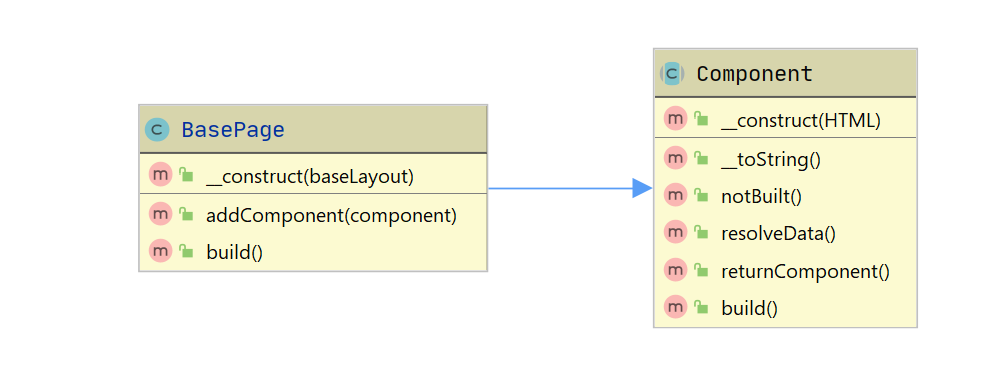
\includegraphics[scale=0.6]{Component.png}

        \caption{Component e BasePage.}
    \end{figure}

    \subsubsection{VO}
    Interfaccia che definisce i contratti di un oggetto rappresentabile virtualmente come istanza di un oggetto remoto, nel nostro caso un elemento istanziato da istanziare nel database.
    Ad esso è sempre associato un corrispettivo DAO che gestisce la comunicazione con il database. Interfaccia pubblica:
    \paragraph{\texttt{arrayDump():Array<String, Any>}} Crea una copia dei valori del VO in un array associativo, i relativi VO contenuti vengono a lora volta dumpati durante la procedura in modo opportuno.
    \paragraph{\texttt{smartDump(Boolean):Array<String, Any>}} Restituisce i valori dell'ogetto come rappresentazione accurata di un record del database, prende in input se non considerare la chiave primaria o meno della tabella.
    \paragraph{\texttt{varDumps(Boolean):Array<String, Any>}} Restituisce un array di tutti i valori dell'oggetto, prende in input se non considerare la chiave primaria .


    \subsubsection{DAO}
    Il DAO come già anticipato si occupa del reperimento e memorizzazione di un corrispettivo tipo di VO nel database. L'interfaccia pubblica:
    \paragraph{\texttt{abstract getAll():Array<VO>}} Ottiene tutti i record rappresentabili dal VO del quale è specializzato costruendoli.
    \paragraph{\texttt{abstract get(Any):VO}} Restituisce il record dalla chiave dello stesso valore dell'input, se non trova un match ritorna un VO vuoto.
    \paragraph{\texttt{abstract delete(VO):Boolean}} Elimina un oggetto dal database, ritorna l'esito dell'operazione.
    \paragraph{\texttt{createAction(Array,String, String):String}} Prepara un'azione da eseguire creando il testo di query e ritornandolo, prende in input i dati di query, il nome della procedura o l'espressione dell'esecuzione e il tipo di chiamata.
    \paragraph{\texttt{abstract save(VO):Boolean}} Salva un elemento sul database, ritorna l'esito dell'operazione.
    \paragraph{\texttt{abstract checkId(VO):Boolean}} Ritorna vero se l'id dell'oggetto virtuale è memorizzato nel database, falso altrimenti.

    \begin{figure}[htbp]
        \label{fig:Dao}
        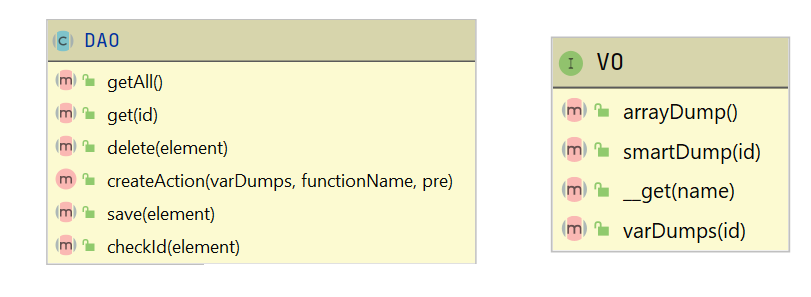
\includegraphics[scale=0.6]{DAO.png}

        \caption{DAO e VO.}
    \end{figure}

    \subsubsection{Le varie Componenti}
    Per brevità verranno elencati solo i componenti principali.

    \paragraph{AdminPanel} Rappresenta il pannello di amministrazione. Consente di effettuare operazioni CRUD su diverse tabelle. È presente un menù laterale a sinistra, nel quale sono elencate le voci possibili. Premendo su una voce il componente carica l'elenco di tutte le entry nel database su quella tabella. Da qui è possibile:
    \begin{itemize}
        \item Inserire una nuova entry;
        \item Modificare una entry;
        \item Eliminare una entry.
    \end{itemize}
    Inserimento e modifica porteranno alla form specifica per il componente, mentre invece l'eliminazione porterà ad una pagina di riepilogo per poter essere confermata.

    \paragraph{PostPage}
    La pagina di un avvistamento è una semplice pagina con dei placeholder valorizzati. Sono presenti uno slideshow in CSS puro delle immagini caricate e una form di inserimento di commenti.

    \paragraph{Feed}
    La pagina principale contiene il \textit{feed}, che è composto dagli avvistamenti inseriti dagli utenti.
    Il feed è ordinabile per tre categorie, quattro se si è autenticati,  l'ordinamento avviene mediante una GET passando
    come parametro il nome del campo da utilizzare per l'ordinamento.

    I filtri sono: \emph{Popolari, Recenti, Discussi, Amici}.

    \paragraph{Card}
    La singola Card è un semplice componente con dei placeholder, pensato per essere messo in grandi quantità all'interno di una pagina.

    \paragraph{Profile}
    Componente che rappresenta il profilo utente mostrandone le informazioni, la sua foto profilo, la lista dei suoi amici e i suoi avvistamenti.

    \paragraph{NewPost}
    Il componente di inserimento di un avvistamento consiste in una semplice form per inserire i dati, controllati da alcune funzioni di filtro .

    \paragraph{GenericBrowser}
    Browser per Card, costruito partendo da un array di oggetti, che
    fornisce un supporto alla navigazione per tanti elementi.

    \subsubsection{Altro}
    Sono anche presenti dei file PHP di supporto, come il file standardLayoutIncludes.php e il file filters.php. Il primo contiene un elenco di import comune a tutte le pagine, ovvero per i componenti dell'intestazione, della \textit{breadcrumb} e della pagina di standard layout. Il secondo, invece, contiene alcune funzioni utili per filtrare le stringhe da inserire nel database.

    \subsection{Javascript}
    Ci sono due file javascript:

    \paragraph{script.js} Questo file viene eseguito alla fine del caricamento di ogni pagina e fa due cose:
    \begin{itemize}
        \item Cerca delle table all'interno della pagina, e se ne trova aggiunge ad essa un bottone che potrà essere usato per ordinare le voci della tabella in base al valore di quella colonna;
        \item Controlla se nella pagina c'è un elemento input di password, e se lo trova aggiunge ad esso un bottone che consente di visualizzare e nascondere la password inserita.
    \end{itemize}

    \paragraph{Validator.js} Questo file viene caricato nell'header della pagina e fornisce una serie di funzioni per la validazione di diverse form.


    \section{Test di accessibilità}
    Per effettuare i test di accessibilità sono stati usati gli strumenti offerti dall'estensione Web developer toolbar\footnote{https://chrispederick.com/work/web-developer/}:
    \begin{itemize}
        \item HTML: https://validator.w3.org/nu/
        \item CSS: http://jigsaw.w3.org/css-validator/
    \end{itemize}

    La validazione HTML riporta alcuni warning, ma sono perlopiù di "utilizzo improprio" dell'attributo \texttt{aria-label}; tali presunti utilizzi impropri sono stati controllati a mano e verificati conformi all'informazione.
    \\ 
    I test sui colori sono stati effettuati con il sito Contrast Checker\footnote{https://webaim.org/resources/contrastchecker/}. Questi test rispettano gli standard WCAG AAA.
    \begin{center}
    \begin{tabular}{c|c|c}
    Sfondo & Testo & Rapporto \\
    \hline
    rgba(30,33,41) & rgba(255,255,255) & 16.09:1 \\
    rgba(73,76,83) & rgba(255,255,255) & 8.59:1 \\
    rgba(179, 220, 253) & rgba(0,0,0) & 14.57:1 \\
    rgba(102, 185, 253) & rgba(0,0,0) & 9.92:1 
    \end{tabular}
\end{center}
    \section{Fonti}
    Per le statistiche sulla diffusione del BirdWatching negli U.S.A:
    \begin{itemize}
        \item  \href{https://chirpbirding.com/blog/111/what-is-the-average-age-of-birdwatchers/}{\emph{What is the average age of birdwatchers?}}, John White, 9 Ottobre 2019
        \item  \href{https://www.americasstateparks.org/birding-a-popular-past-time/}{\emph{Birding a popular past time}}, America's State Parks
    \end{itemize}
    Lista rossa e IUCN per il pericolo di estinzione:
    \begin{itemize}
        \item \href{http://www.iucn.it/liste-rosse-cosa-sono.php}{\emph{Cosa sono le Liste Rosse}}, IUCN
    \end{itemize}
    Le immagini caricate sul sito, sia di uccelli, che dei profili degli utenti, sono immagini a licenza libera, prelevate da questi due siti:
    \begin{itemize}
        \item https://wikipedia.org 
        \item https://www.pexels.com/it-it/license/    
    \end{itemize}

\end{document}